\section{The Methodological Approach}

% - proviamo le features handcrafted
% - cerchiamo di migliorarle con le cnn
%     - from scratch (come nel paper)
%     - data augmentation
%     - features extraction (con reti pretrainate)

\subsection{Handcrafted Features}
The first model tested was a simple neural network on handcrafted features of the small subset.
% Next, a CNN model was tested to try to improve the performance of the handcrafted one.

The split of the data was the same as that provided by the dataset (6400 train, 800 validation and 800 test).
The number of features was 518. The features were standardized on the statistics of the training set.

The architecture of the neural network was found by testing a different number of neurons for two layers.
The best parameters found were (512, 256).
Adam was used as an optimizer with a learning rate of 0.0001 and a batch size of 32.

\subsection{Convolutional Neural Network}
According to the state of the art\cite{zeng2019spectrogram}, the approach that now seems to perform better for these tasks is the one based on spectrograms and Convolutional Neural Networks.

The architecture used was the one suggested by "Daniel Kostrzewa" \cite{kostrzewa2021music}.
"Layer 1 and 2 have both 64 kernels each, whereas layers 3 and 4 have 128 kernels. The kernel size of all layers is equal to 5. After each layer, there is 2-D max pooling applied with kernel size and stride equal 2. In every convolutional layer, ReLU is used as an activation function. Batch normalization is performed afterward. The convolutional layers are followed by one fully connected linear layer with linear activation function and the final output of 8 nodes" \cite{kostrzewa2021music}. Dropout probability was 0.20. The number of trainable parameters was 735 944.

\begin{figure}[ht]
    \centering
    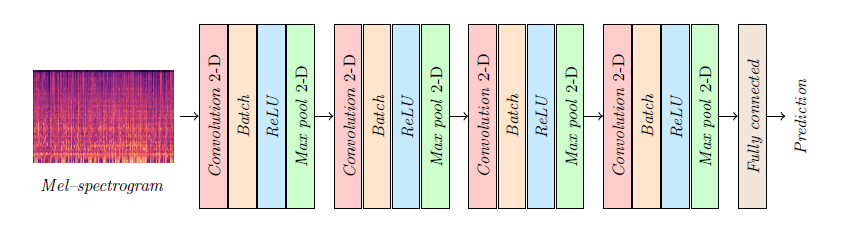
\includegraphics[scale=0.6]{images/CNN-architecture.png}
    \caption{The architecture suggested by "Daniel Kostrzewa" \cite{kostrzewa2021music}.}
    \label{fig:CNN-architecture}
\end{figure}

An hyper-parameter optimization was performed on this architecture.
Not being able to do an optimization from start to finish and on all the hyper-parameters space,
it was decided to use Hyperband \cite{li2016novel} and to optimize only some hyper-parameters.

The hyper-parameters considered for the optimization were:
\begin{itemize}
    \item The size of the kernel (fixed on each layer) in [3,6].
    \item The number of kernels for each layer in [32, 256].
    \item The probability of dropout in \{0.2, 0.25, 0.5\}.
    \item The initial learning rate in \{0.01, 0.001, 0.0001\}.
\end{itemize}

The optimization of the network led to have, in the case without date augmentation, the first layer with 32 kernels, the second one with 128, the third with 192 and the fourth with 98. The kernel size of all layers was equal to 6.
Dropout probability was 0.25 and initial learning rate was 0.001.

While in the case with data augmentation the optimization led to have, the first layer, the second and the third all with 64 kernels and the fourth with 96.
The kernel size of all layers was equal to 4. Dropout probability was 0.25 and initial learning rate was 0.0001.

\subsection{Feature extraction with CNN}
Later the approach was changed to using transfer learning as the amount of data is not large.

A features extraction process was applied. Two Top-5 CNN architectures trained on ImageNet were chosen: VGG16 and ResNet50. These architectures are similar in accuracy, but different in the number of parameters.

Since the considered domain differs from ImageNet's natural images, it is expected that lower levels should perform better.

\vspace{5mm}
\noindent
The characteristics were extracted in different cut levels and each vector was standardized and then a PCA (Principal Component Analysis) was applied in order to reduce the high dimensionality due to the lower layers.

\noindent
Different values of explained variance percentage were tested on the fc2 layer of VGG16: 99\%, 95\%, 90\%.

\noindent
After the results were obtained it was found out that PCA 90\% was the best. 
Then several cut levels were tried for VGG16 (\text{block5\_pool}, fc1, fc2) and for ResNet50 (\text{conv5\_block1\_2\_relu}, \text{avg\_pool})

\noindent
For computational reasons no tests were performed without PCA and at much lower levels.

\vspace{5mm}
\noindent
For this phase, the training and validation data were combined to then carry out a k-fold cross-validation with the grid search to fine-tune the machine learning models.

\noindent
Different standard classifiers were tried, linear SVM, SVM with kernel RBF and a MLP(Multi Layer Perceptron).

\noindent
The hyper-parameters considered was:
\begin{itemize}
    \item C: [0.01, 0.1, 1, 10] (Linear SVM).
    \item C: [0.01, 0.1, 1, 10], gamma: [0.01, 0.001, 0.0001] (SVM RBF).
\end{itemize}

\noindent
For the Multi Layer Perceptron the Adam optimizer was used with a batch size of 32 and a learning rate of 1e-4. The number of epochs was set to a max of 200 and early stopping was also used. 
All layers use a relu activation function, while the last layer was a Softmax and a Cross Entropy Loss was used.
\begin{itemize}
    \item network architectures: [(512, 256), (512, 32), (512,)],
    \item l2 regularization alpha: [0.01, 0.03, 0.05]
\end{itemize}
